\documentclass{article}

\usepackage[utf8]{inputenc}
\usepackage[brazilian]{babel}
\usepackage{graphicx}
\usepackage{float}
\usepackage[pdftex]{hyperref}
\usepackage{epstopdf}
\usepackage{etoolbox}
\usepackage{amsmath}
\usepackage{amsfonts}
\usepackage{amssymb}
\usepackage{caption}
\usepackage{subcaption}
\usepackage{setspace}
\usepackage{tikz}

\patchcmd{\thebibliography}{\section*}{\section}{}{}
\newcommand{\R}{\ensuremath{\mathbb{R}}}
\newcommand{\Prob}{\ensuremath{\mathbb{P}}}
\newcommand{\K}{\ensuremath{\mathbb{K}}}
\newcommand{\U}{\ensuremath{\mathbb{U}}}
\newcommand{\N}{\ensuremath{\mathbb{N}}}
\newcommand{\Lg}{\ensuremath{\mathbb{L}}}
\newcommand{\T}{\ensuremath{\rm Tr}}
\newcommand{\sg}{{\sigma(x_k)}}

\newcommand{\G}{\ensuremath{\mathcal{G}}}
\newcommand{\F}{\ensuremath{\mathcal{F}}}
\newcommand{\C}{\ensuremath{\mathcal{C}}}
\newcommand{\E}{\ensuremath{\mathcal{E}}}
\newcommand{\Hn}{\ensuremath{\mathcal{H}}}
%\newcommand{\Hoo}{\ensuremath{\mathcal{H}_\infty}}
\newcommand{\Hop}{\ensuremath{\mathcal{H}_{op}}}
% --------------------------------------------------
\newtheorem{theo}{Teorema}
\newtheorem{exa}{Exemplo}
\newtheorem{lemm}{Lema}
\newtheorem{coro}{Corolário}
\newtheorem{defn}{Definição}[section]

%opening


\begin{document}

\begin{titlepage}
\begin{center}

\newcommand{\HRule}{\rule{\linewidth}{0.5mm}}
% Upper part of the page. The '~' is needed because \\
% only works if a paragraph has started.

\includegraphics[width=0.15\textwidth]{logoUnicamp}~\\[1cm]

\textsc{\LARGE Universidade Estadual de Campinas}\\[1.5cm]

\textsc{\Large Faculdade de Engenharia Mecânica}\\[0.5cm]

% Title
\HRule \\[0.4cm]
{ \huge \bfseries ES670 - Projeto de Sistemas Embarcados\\ \vspace{1cm} Relatório - Projeto Prático (Parte 1/7) \\
\Large{Requisitos de Teclado, LEDs e Display de Sete Segmentos} \\[0.4cm] }

\HRule \\[1.5cm]

% Author and supervisor
\begin{minipage}{0.6\textwidth}
\begin{flushleft} \large
\emph{Nome:}\\
Rodolfo Nobre Bitu de Morais\\Guilherme de Oliveira Souza\\ Marcelli Tiemi Kian
\end{flushleft}
\end{minipage}
\begin{minipage}{0.2\textwidth}
\begin{flushright} \large
\emph{RA}\\ 105654\\117093\\
117892
\end{flushright}
\end{minipage}

\vfill

% Bottom of the page
{\large \today}

\end{center}
\end{titlepage}


\onehalfspacing
\section{Objetivo} 
O objetivo do projeto é, de maneira incremental, implementar no target os requisitos apresentados no roteiro\cite{bb:roteiro} inicialmente desenvolvendo o modelo e depois implementando cada requisito. Estes requisitos são referentes à configuração e implementação de: entradas de teclado, acionamento de LEDs, display de sete segmentos, protocolo de comunicação, display LCD, medição de velocidade de rotação, PWM, ADC, controlador. 
	
\section{Modelagem}
% Diagramas requisitos implementados, digrama de blocos, etc
Utilizando o Rational Rhapsody Modeler e tomando como base os requisitos propostos mostrados na figura \ref{fig:requisitos}, complementamos o modelo inicial (requisitos de teclado e LEDs) adicionando um bloco ao modelo referente aos displays de sete segmentos (REQ1C), conforme mostrado na figura \ref{fig:blocos}.

O bloco SevenSeg possui três operações: inicialização, definição de saída (recebendo qual dos displays será usado e qual valor deve ser exibido) e definição de saída com inteiro (recebendo apenas o valor inteiro a ser exibido no conjunto de quatro displays).
\begin{figure}[H]
	\centering
	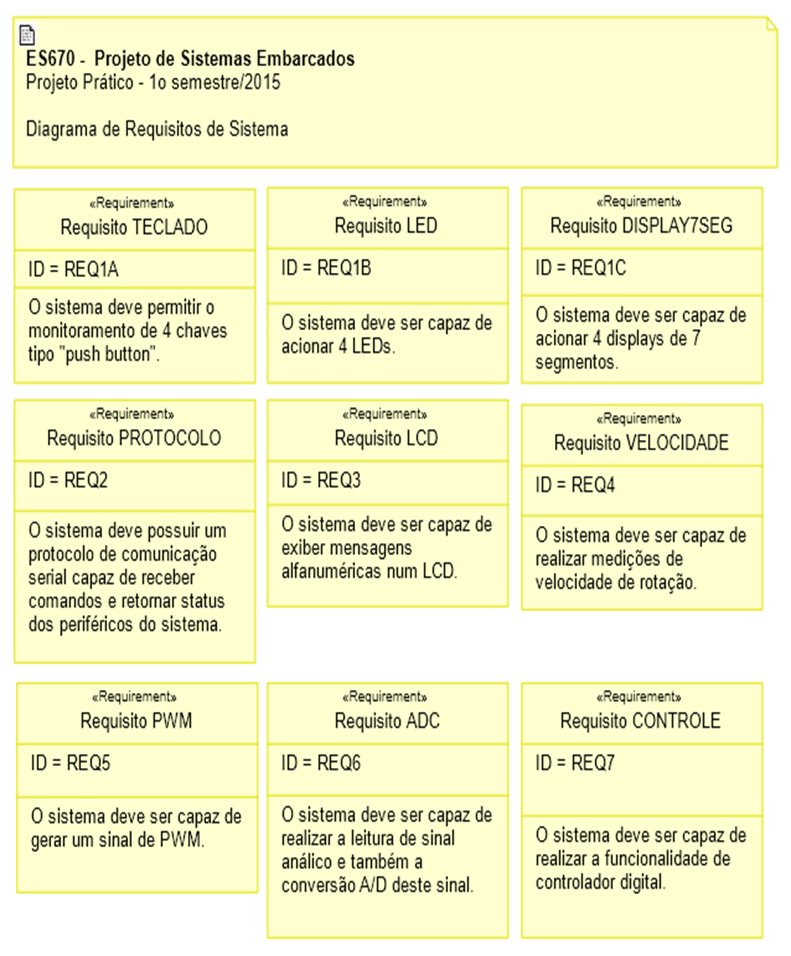
\includegraphics[width=0.7\linewidth]{requisitos}
	\caption{Diagrama de requisitos}
	\label{fig:requisitos}
\end{figure}
\begin{figure}[H]
	\centering
	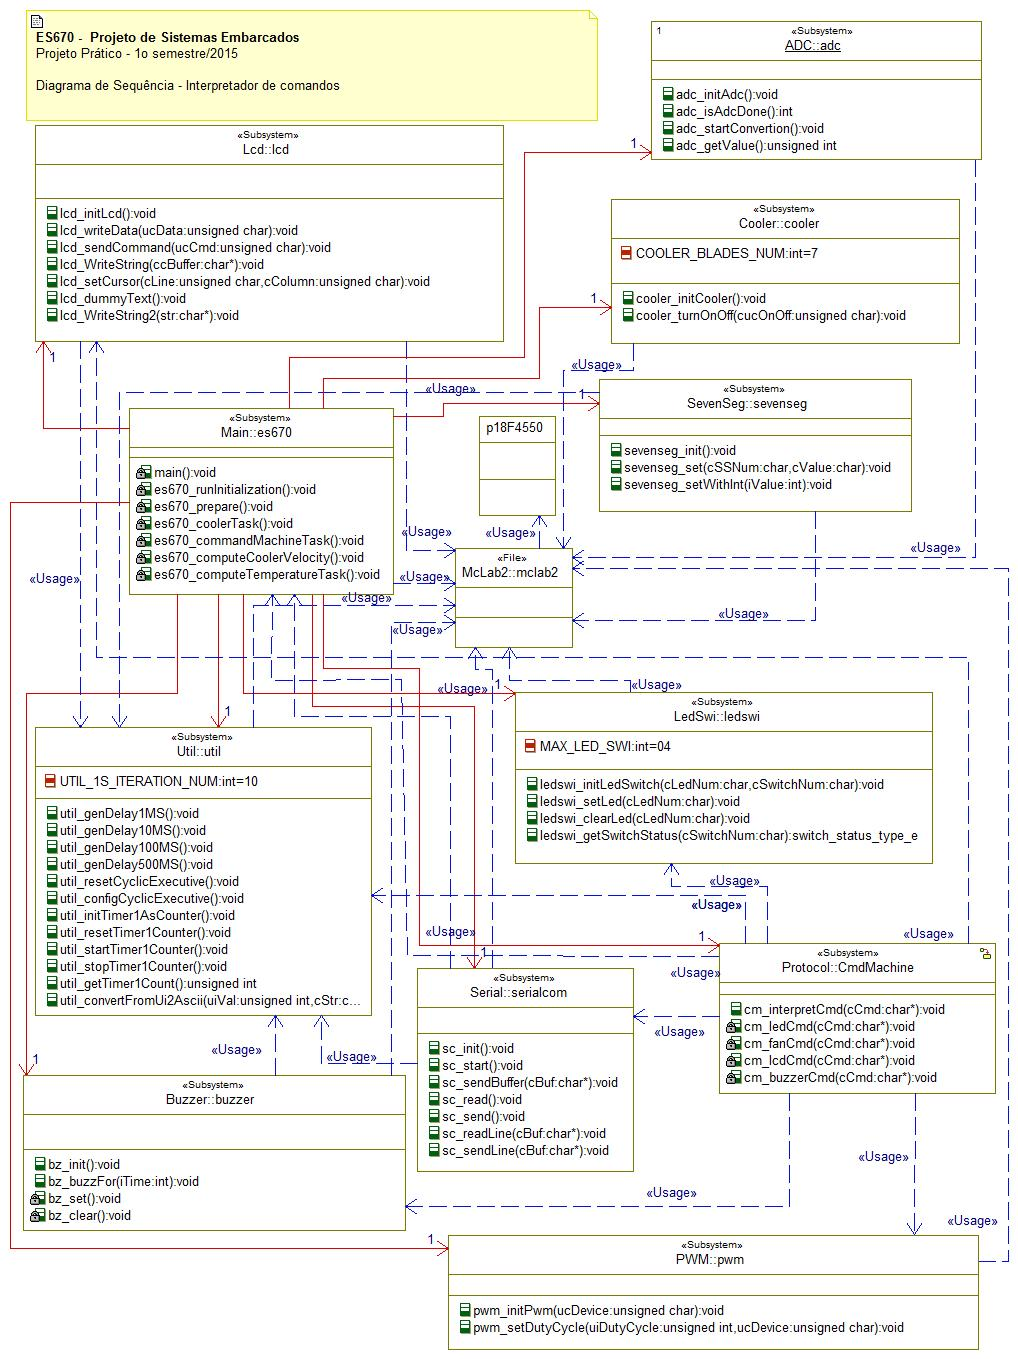
\includegraphics[width=0.9\linewidth]{blocos}
	\caption{Diagrama de definição de blocos}
	\label{fig:blocos}
\end{figure}

\section{Diagramas Esquemáticos}
% Diagramas esquemáticos do target utilizados

\begin{figure}[H]
	\centering
	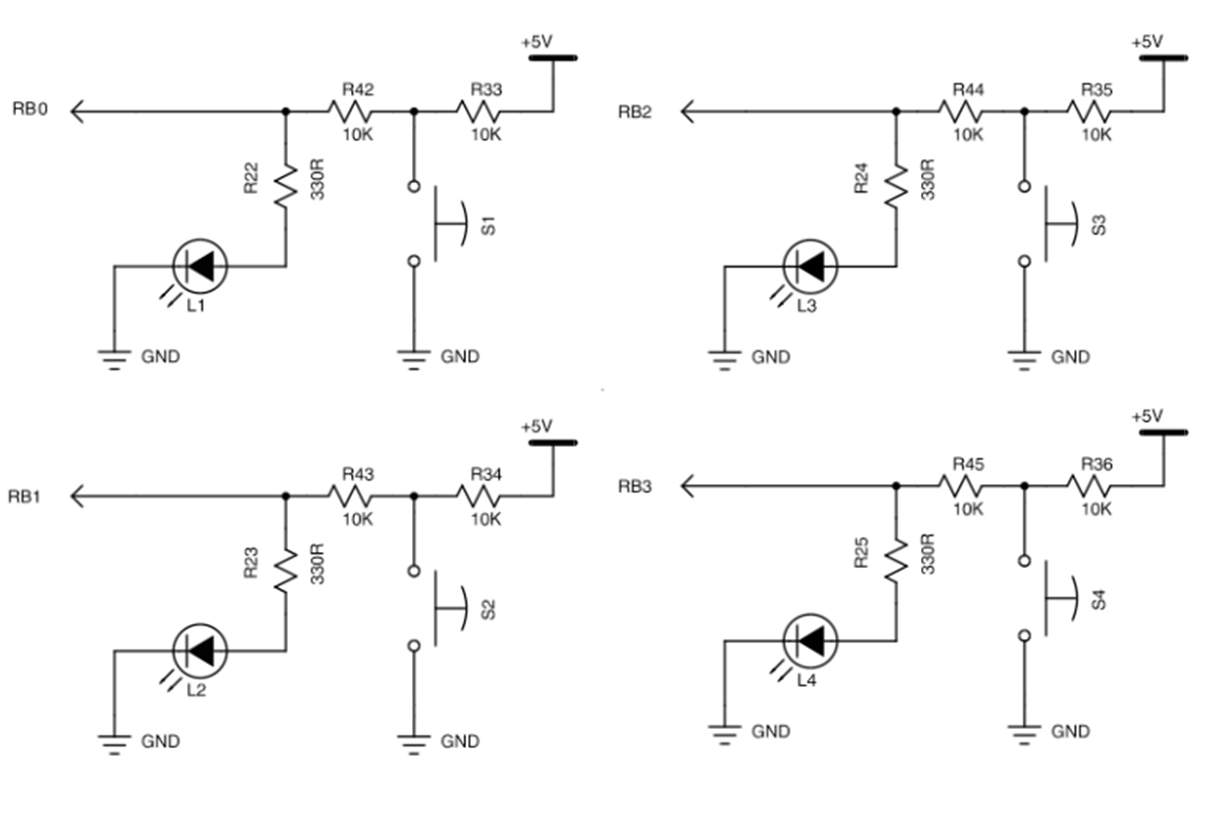
\includegraphics[width=0.7\linewidth]{esq_ledswi}
	\caption{Esquema teclado e LEDs}
	\label{fig:esq_ledswi}
\end{figure}
\begin{figure}[H]
	\centering
	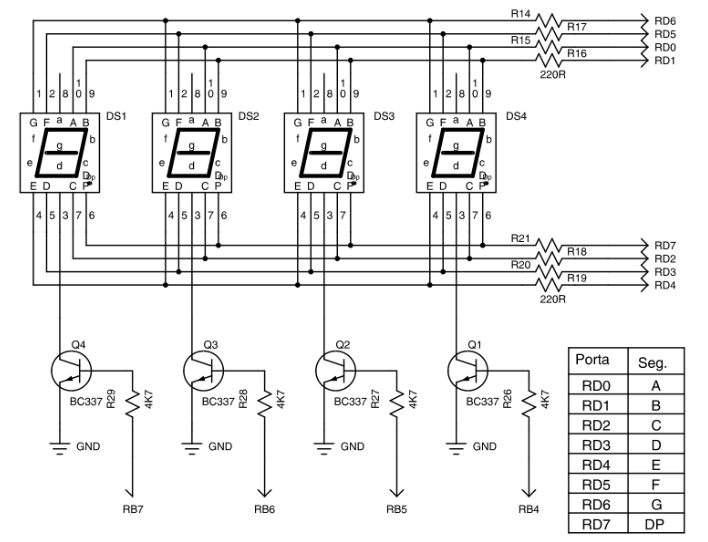
\includegraphics[width=0.9\linewidth]{esq_7seg}
	\caption{Esquema sete segmentos}
	\label{fig:esq_7seg}
\end{figure}
Como pode ser visto na figura \ref{fig:esq_7seg}, é necessário fazer um gerenciamento das portas RB4-7 e RD0-7 para que sejam mostrados os valores desejados nos displays de sete segmentos. Para isso, é preciso alternar qual RB está ativo fazendo a mudança nos RD0-7 para que cada display esteja mostrando um valor diferente. É importante lembrar que a frequência dessa alternância seja escolhida de modo que o olho humano não perceba que os displays estão ligando e desligando.


\section{Matriz de Rastreabilidade}
% Matriz de rastreabilidade de requisitos vs implementações
\begin{table}[H]%TODO
	\centering
	\caption{Matriz de Rastreabilidade}
	\label{tab:rastreabilidade}
	\begin{tabular}{|c|c|}
		\hline ID do Requisito & Implementação \\ 
		\hline REQ1A 	& \\ 
						& \\
						& \\
		\hline REQ1B 	& \\ 
		\hline REQ1C 	& \\ 
		\hline 
	\end{tabular} 
\end{table}
\section{Notas}
% Dificuldades, observações relevantes, correções, ...

Os maiores problemas identificados foram a dificuldade de conseguir conectar a placa com o computador e alguns mal contatos relacionados aos botões e do próprio PIC. Além disso, houve alguns conflitos com a IDE, pois muitas funcionalidades poderiam ter sido implementadas, já que a função de auto-completar é bem comum em IDE's e o duplo clique poderia selecionar a palavra em vez de colocar um breakpoint.


\section{Apêndice}
% Colocar como apêndice toda a listagem do código fonte
	
\begin{thebibliography}{widestlabel}
	\bibitem{bb:roteiro}{Roteiro de Laboratório - Semanas 04 e 05 (disponibilizado para os alunos)}
\end{thebibliography}
\end{document}

